\section{Teste}\label{teste}

\subsection{Equações}\label{sec:sec1}

\[\eqlabel{eq:raoult} 
    \boxed{
        \text{Lei de Raoult:}
        \quad
        P = P_\text{sat} x_\text{solvente}
    }
\]

Essa é a \eqref{eq:raoult} da seção \secref{sec:sec1}

\subsection{Figuras}\label{figuras}

\subsubsection{Imagem}\label{imagem}

Figura sem legenda:

\begin{figure}
\hypertarget{fig:latex}{%
\centering
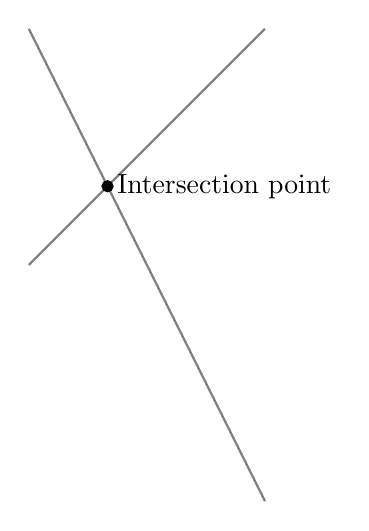
\begin{tikzpicture}
  \draw[gray, thick] (-1,2) -- (2,-4);
  \draw[gray, thick] (-1,-1) -- (2,2);
  \filldraw[black] (0,0) circle (2pt) node[anchor=west]{Intersection point};
\end{tikzpicture}
\caption{Figura em latex.}\label{fig:latex}
}
\end{figure}

\subsubsection{Imagem}\label{imagem-1}

Figura sem legenda:

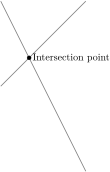
\includegraphics{img/image.png}

\subsubsection{Figura com legenda}\label{figura-com-legenda}

Figura com legenda:

\begin{figure}
\hypertarget{fig:fig1}{%
\centering
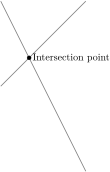
\includegraphics{img/image.png}
\caption{Legenda da figura.}\label{fig:fig1}
}
\end{figure}

Essa é a \figref{fig:fig1}.

\subsubsection{Figura de página inteira (TODO)}\label{figura-de-puxe1gina-inteira-todo}

Figura na página inteira:

\begin{figure}
\hypertarget{fig:fig2}{%
\centering
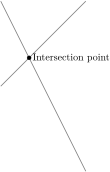
\includegraphics{img/image.png}
\caption{Legenda da figura de página inteira}\label{fig:fig2}
}
\end{figure}

Essa é a \figref{fig:fig2}.

\subsubsection{Tikz}\label{tikz}

Uma figura:

\includesvg{img/1T01img01.svg}

E outra figura:

\includesvg{img/1T01img02.svg}

\subsection{Tabelas}\label{tabelas}

\subsubsection{Tabela sem legenda}\label{tabela-sem-legenda}

\begin{tblr}{X[3.0,l]X[2.0,r]X[1.0,c]}
x &  Olá &  Tchau\\
Elemento 1 & 1 1 & não é o \(\ce{H2SO4}\)\\
Molécula & 2 1 & \(\ce{NaOH}\) 1
\end{tblr}

\subsubsection{Tabela com legenda}\label{tabela-com-legenda}

Tabela com legenda:

\begin{table}[label=tbl:tbl1]{Legenda com equação \(x^2\)}

\begin{tblr}{X[1.0,l]X[2.0,r]X[3.0,c]}
x &  Olá &  Tchau\\
Elemento 1 & 1 1 & não é o \(\ce{H2SO4}\)\\
Molécula & 2 1 & \(\ce{NaOH}\) 1
\end{tblr}

\end{table}

Essa é a \tblref{tbl:tbl1}.

\subsection{Ambientes curtos}\label{ambientes-curtos}

Esse é um warning:

\begin{warning}{Atenção}

Presta atenção nessa parada!

\end{warning}

\subsection{Ambientes longos}\label{ambientes-longos}

Esse é um exemplo:

\begin{example}{Cálculo do comprimento de onda da luz a partir da frequência}

\textbf{Calcule} o comprimento de onda da luz vermelha, de frequência \(\pu{4,3e14 Hz}\).

\step{Use a relação entre frequência e comprimento de onda da radiação.}

De \(\lambda = c/f\) \[
    \lambda = \dfrac{ \pu{3e8 m.s-1} }{ \pu{4,3e14 Hz} } = \boxed{ \pu{700 nm} }
\]

\end{example}

Esse exemplo, o exemplo 1, é pica dms!

\subsection{Resumo}\label{resumo}

\begin{quote}
Esse é resumo do final da seção!
\end{quote}